\section{Data and the leak-free telemetry window}
\label{sec:data}

\subsection{The trace and the label}
We use the Alibaba cluster-trace-gpu-v2020 release~\cite{weng2022mlaas}, distributed under the CC BY 4.0 licence. It covers \V{data.span.days} days of Alibaba's PAI machine-learning platform; timestamps are seconds from an undisclosed origin. The task table holds \V{data.raw.tasks} tasks. We treat \texttt{Failed} as the positive class and \texttt{Terminated} as the negative class and drop the \V{data.raw.unresolved} tasks (\V{data.raw.unresolvedshare}) whose status is \texttt{Running} or \texttt{Waiting}, which leaves \V{data.lab.tasks} labelled tasks with a failure rate of \V{data.lab.rate}. The submitting user comes from the job table and serves only as a split key; it is never a model input and appears in no exported file.

\subsection{Why the task's own telemetry cannot be used}
The obvious way to attach machine telemetry to a task is to average the telemetry of the worker that ran it over the task's lifetime. In this trace the machine-metric table has rows for \V{data.cov.term} of the instances of terminated tasks and for \V{data.cov.fail} of the instances of failed ones, and \V{data.noend.fail} of failed instances have no end time. A worker-keyed join therefore keeps almost no failures, and a model trained on it would learn that the presence of telemetry implies success. This is a leakage path and a coverage gap at once~\cite{kaufman2012leakage,kapoor2023leakage}.

\subsection{The leak-free window}
We therefore describe the machine instead of the task. For each task we take the machine of its first instance (earliest start, ties broken by file order) and average the machine-metric rows of \emph{other} jobs' workers on that machine whose end time falls in the hour before the task started. Two rules make the window leak-free: no row that ends at or after the task's start is used, and no row of the task's own job is used (Figure~\ref{fig:pipeline}). The ten features are the four resource requests of the task (\feat{plan_cpu}, \feat{plan_mem}, \feat{plan_gpu}, \feat{inst_num}), the GPU count of the machine (\feat{cap_gpu}) and five window averages (\feat{avg_cpu_usr}, \feat{avg_gpu_util}, \feat{avg_cpu_kernel}, \feat{avg_load_1}, \feat{avg_net_receive}). A task with any missing feature is dropped. The window length is the only free parameter of the build; \SecRef{sec:res-lookback} varies it.

% Pipeline and leak-free window (TikZ). Shared by main.tex and ieee/main_ieee.tex; the width follows \linewidth.
\begin{\pipelinefig}[t]
\centering
\resizebox{\linewidth}{!}{%
\begin{tikzpicture}[
  font=\sffamily\small,
  box/.style={draw=black!70, rounded corners=2pt, fill=black!4, align=center, minimum height=9mm, inner sep=3pt},
  arr/.style={-{Stealth[length=2.2mm]}, black!70, thick},
  lbl/.style={font=\sffamily\scriptsize, black!70, align=center}]
% ---------------------------------------------------------------- join path
\node[box, text width=24mm] (task) {task table\\{\scriptsize request, label}};
\node[box, text width=24mm, right=14mm of task] (inst) {instance table\\{\scriptsize first instance}};
\node[box, text width=24mm, right=14mm of inst] (mm) {machine metrics\\{\scriptsize other jobs, window}};
\node[box, text width=22mm, right=12mm of mm] (spec) {machine spec\\{\scriptsize \texttt{cap\_gpu}}};
\node[box, text width=22mm, below=6mm of task] (job) {job table\\{\scriptsize user: split key}};
\node[box, text width=40mm, below=6mm of mm, xshift=-10mm, fill=black!10] (feat) {10 features, label, start time\\{\scriptsize no clipping in the build}};
\draw[arr] (task) -- node[lbl, above] {job, task} (inst);
\draw[arr] (inst) -- node[lbl, above] {machine, $t_0$} (mm);
\draw[arr] (mm) -- node[lbl, above] {machine} (spec);
\draw[arr] (task) -- (job);
\draw[arr] (inst.south) |- (feat.west);
\draw[arr] (spec.south) |- (feat.east);
% ---------------------------------------------------------------- the window on a time axis
\begin{scope}[xshift=153mm, yshift=4mm]
  \draw[-{Stealth[length=2mm]}, black!70] (0,-6mm) -- (62mm,-6mm) node[right, lbl] {time};
  \fill[black!8] (14mm,-14mm) rectangle (44mm,10mm);
  \draw[black!60, dashed] (14mm,-14mm) -- (14mm,10mm) node[above, lbl] {$t_0-1\,$h};
  \draw[black!80, thick] (44mm,-14mm) -- (44mm,10mm) node[above, lbl] {$t_0$ (task start)};
  % metric rows plotted at their end time
  \foreach \x/\kind in {8/out, 20/in, 27/in, 33/own, 39/in, 44/edge, 52/out} {
    \ifthenelse{\equal{\kind}{in}}{\fill[black!85] (\x mm,0) circle (1.3mm);}{}
    \ifthenelse{\equal{\kind}{out}}{\draw[black!60] (\x mm,0) circle (1.3mm);}{}
    \ifthenelse{\equal{\kind}{edge}}{\draw[black!60] (\x mm,0) circle (1.3mm);}{}
    \ifthenelse{\equal{\kind}{own}}{\draw[black!80, thick] (\x mm-1.2mm,-1.2mm) -- (\x mm+1.2mm,1.2mm) (\x mm-1.2mm,1.2mm) -- (\x mm+1.2mm,-1.2mm);}{}
  }
  \node[lbl, anchor=north west] at (0mm,-15mm) {\tikz\fill[black!85] (0,0) circle (1.1mm); other job, ended in window: averaged\quad
     \tikz\draw[black!80, thick] (-1mm,-1mm) -- (1mm,1mm) (-1mm,1mm) -- (1mm,-1mm); task's own job: excluded};
  \node[lbl, anchor=north west] at (0mm,-20mm) {\tikz\draw[black!60] (0,0) circle (1.1mm); ended before the window or at/after $t_0$: excluded};
\end{scope}
\end{tikzpicture}}
\caption{Left: the join path from the raw tables to the feature matrix. The user joins only as a split key. Right: the leak-free window. For a task that starts at $t_0$, the five telemetry features average the machine-metric rows of other jobs' workers on the task's machine that ended in $[t_0-1\,\mathrm{h},\, t_0)$; rows of the task's own job and rows ending at or after $t_0$ are never used.}
\label{fig:pipeline}
\end{\pipelinefig}


\subsection{The full trace and the original sample}
The first version of this study built its matrix from a stratified sample of \V{data.v1.sample} labelled tasks and kept the \V{data.orig.tasks} that survived the rules. Here we apply the same rules to every labelled task. Caching the instance table once and computing the windows with vectorised searches makes the build take \V{data.build.minutes} minutes on a laptop with \V{data.ram} of memory. Table~\ref{tab:attrition} and Figure~\ref{fig:attrition} give the attrition: \V{data.full.tasks} tasks survive (\V{data.full.share} of the labelled tasks), with \V{data.full.fail} failures (\V{data.full.rate}) from \V{users.full.users} users. Two steps remove almost all of the lost tasks. At the telemetry step \V{data.tele.nowindow} tasks are lost because no other job's metric row ended on their machine in the window, \V{data.tele.nomachine} because their machine has no telemetry at all, and \V{data.tele.other} because their first instance never started or has no machine. At the last step \V{data.missing.tasks} tasks are lost because a telemetry value is missing. The failure rate rises from \V{data.lab.rate} to \V{data.full.rate} along the way, so the surviving tasks are a selected population. Taking the original \V{data.orig.tasks} tasks from the full build reproduces the first version's matrix value for value before clipping (largest relative difference \V{data.v1.maxrel}), and the same holds for its four other lookback windows. We keep those tasks as the \emph{original sample}, so every protocol can be compared with the first version.

% Generated by scripts/paper_tables.py. Do not edit.
\begin{table}[t]
\centering
\small
\TabCaption{tab:attrition}{Attrition of the full trace at a 1\,h lookback}{Each row is the number of tasks that pass every step up to and including it. A task can lack several features at once, so the counts of missing features overlap.}
\begin{tabular}{@{}lrr@{}}
\toprule
Step & Tasks & Failure rate \\
\midrule
Task table & 1,261,050 &  \\
Labelled (Failed or Terminated) & 1,141,835 & 22.5\% \\
First instance found & 1,141,835 & 22.5\% \\
Telemetry from other jobs in the window & 791,592 & 26.5\% \\
Machine in the specification table & 791,592 & 26.5\% \\
No missing feature & 539,816 & 27.4\% \\
\midrule
\multicolumn{3}{@{}l}{\emph{Lost at the telemetry step}} \\
\quad no other job's row ended in the window & 306,674 & \\
\quad machine has no telemetry at all & 43,537 & \\
\quad first instance never started & 31 & \\
\quad first instance has no machine & 1 & \\
\multicolumn{3}{@{}l}{\emph{Missing at the last step (overlapping)}} \\
\quad \feat{avg_load_1} missing & 103,766 & \\
\quad \feat{avg_cpu_kernel} missing & 102,101 & \\
\quad \feat{avg_cpu_usr} missing & 90,482 & \\
\quad \feat{avg_gpu_util} missing & 87,393 & \\
\quad \feat{avg_net_receive} missing & 76,872 & \\
\quad \feat{plan_gpu} missing & 37,914 & \\
\bottomrule
\end{tabular}
\TabNotes
\end{table}


\begin{figure}[t]
\centering
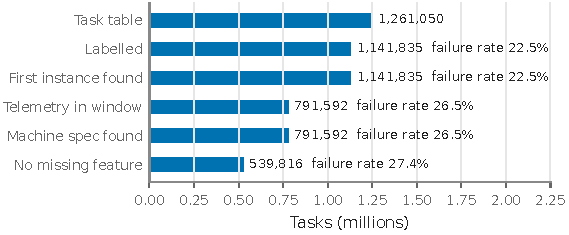
\includegraphics[width=0.62\linewidth]{figures/attrition.pdf}
\caption{Attrition of the full trace at a one-hour lookback: tasks remaining after each step, with the failure rate among them.}
\label{fig:attrition}
\end{figure}

\subsection{Clipping and scaling per split}
The first version clipped every feature at its 1st and 99th percentiles over all rows before splitting, so the clip bounds carried information from the rows that later formed the validation and test sets. In this version the build returns raw values, and each protocol fits the clip bounds and the min-max scaling on its training split alone and applies them unchanged to the validation and test splits. A unit test moves every test row to an extreme value and checks that no fitted constant changes. All models receive identical inputs.

\subsection{Who submits the failures}
Failures are concentrated in a few users (Figure~\ref{fig:concentration}). In the full trace the largest user, User~1, submits \V{users.full.u1.taskshare} of the tasks and \V{users.full.u1.failshare} of the failures, with a failure rate of \V{users.full.u1.rate}. User~4, fourth by task count, submits \V{users.full.u4.taskshare} of the tasks with a failure rate of \V{users.full.u4.rate}. Together the two hold \V{users.full.u14.failshare} of all failures, and the ten users with the most failures hold \V{users.full.top10.failshare}. The original sample has the same structure (User~1: \V{users.orig.u1.taskshare} of the tasks, \V{users.orig.u1.failshare} of the failures). A random task-level split therefore places most of these users' tasks on both sides of the split.

\begin{figure}[t]
\centering
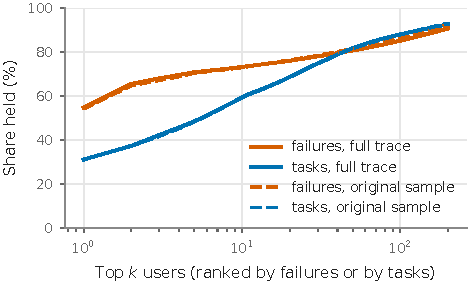
\includegraphics[width=0.62\linewidth]{figures/concentration.pdf}
\caption{Share of all failures (vermillion) and of all tasks (blue) held by the $k$ users with the most failures or the most tasks; full trace solid, original sample dashed. The horizontal axis is logarithmic.}
\label{fig:concentration}
\end{figure}
